\documentclass[12pt,a4paper,oneside]{article}
\usepackage{geometry}
\geometry{
	left=1.5cm, %% canh giữa hình
	right=1.5cm,
	top=2cm,
	bottom=2cm,
}
%ver-texlive2021
\usepackage{amsmath,amssymb,mathrsfs,fancyhdr,enumerate,multirow,makecell,currfile,venndiagram}
\usepackage{tikz-3dplot,tikz,tkz-tab,tabvar}
\usepackage{graphics}
\usepackage{tabularx}
\usetikzlibrary{arrows,calc,intersections,angles,snakes,quotes,backgrounds,shapes.geometric,patterns}
\usepackage{pgfplots}
\pgfplotsset{compat=1.9}
\usepgfplotslibrary{fillbetween}
\usepackage[tikz]{bclogo}
%\usepackage{xcolor}
% \usepackage{tcolorbox}
\usepackage{ex_test}
\usepackage{times}
\usepackage{array}

\setlength{\columnseprule}{1pt} 
\usepackage{tabularx,array}
\usepackage{fancyhdr}
\pagestyle{fancy}
\fancyhead{} 
\fancyfoot{} 
\fancyfoot[C]{Trang \textbf{\thepage}/5} 
\renewcommand{\headrulewidth}{0pt} 
\renewcommand{\nameex}{\color{blue}Câu}

%\usepackage{xcolor}
%\usepackage{tikz}
%
%\newcommand{\circlelabel}[1]{%
%	\tikz[baseline=(c.base)] 
%	\node[draw=blue, circle, inner sep=1pt, line width=0.7pt] (c)
%	{\textcolor{blue}{#1}};%

\renewcommand{\FalseEX}{\stepcounter{dapan}\circled{\textbf{\Alph{dapan}}}}
%\renewcommand{\FalseEX}{\stepcounter{dapan}\circled{\Alph{dapan}}}


\begin{document}
	
	 \begin{minipage}[t]{0.5\textwidth}
		 	\begin{center}
			 	{\bfseries SỞ GD\&ĐT TP. HUẾ\\
				 	TRƯỜNG THPT NGUYỄN CHÍ THANH}\\[-0.6em]
			 \rule{3.6cm}{0.8pt}\\
			 {\itshape (Đề thi gồm có 04 trang)}	
			 	\end{center}
		 \end{minipage}\hfill
	 \begin{minipage}[t]{0.45\textwidth}
		 	\centering
		 	{\bfseries ĐỀ KIỂM TRA THƯỜNG XUYÊN}\\[-0.15em]
		 	{\bfseries NĂM HỌC 2025 -- 2026}\\[-0.15em]
		 	{\bfseries MÔN VẬT LÍ -- Lớp 12}\\[0.25em]
		 	{Thời gian làm bài : 45 phút}\\[-0.15em]
		 	{\itshape (không kể thời gian phát đề)}
		 \end{minipage}
		
\vspace{0.2cm}
%\noindent\rule{\textwidth}{0.5pt}
\noindent\textbf{PHẦN I. Câu trắc nghiệm nhiều phương án lựa chọn.} Mỗi câu hỏi chỉ chọn một phương án.

% Câu 2 (Trang 1)
\begin{ex}
	Nội dung của câu nào sau đây \textbf{không} đúng?
	\choice
	{Trong quá trình đẳng áp, thể tích của một khối lượng khí xác định tỷ lệ với nhiệt độ tuyệt đối}
	{Hệ số nở đẳng áp của mọi chất khí đều bằng $1/273$}
	{Đường biểu diễn quá trình đẳng áp trong hệ tọa độ $(V - T)$ là đường thẳng có đường kéo dài đi qua gốc toạ độ}
	{Trong quá trình đẳng áp, khi nhiệt độ tăng từ $20^\circ\text{C}$ đến $40^\circ\text{C}$ thì thể tích khí tăng gấp đôi}
\end{ex}

% Câu 3 (Trang 1)
\begin{ex}
	\immini{
	Hình bên mô tả quá trình biến đổi trạng thái trong hệ tọa độ (trục tung thể tích của khối khí $V$ – trục hoành nhiệt độ của khối khí $T$) của một lượng khí lí tưởng xác định. Đó là quá trình
	\choice
	{đẳng áp}
	{đẳng nhiệt}
	{đẳng tích}
	{áp suất tăng đều theo thể tích}
	}{
	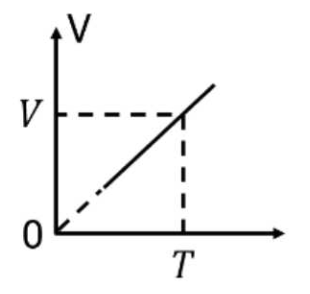
\includegraphics[scale=0.4]{img1/H3.png}
	}
\end{ex}

% Câu 4 (Trang 1)
\begin{ex}
	Ở gần nhiệt độ ngưng tụ, chúng ta không thể coi các phân tử khí ..(1).. được nữa và chất khí ..(2).. tuân theo định luật Boyle hay định luật Charles. Điền các cụm từ thích hợp vào các chỗ trống.
	\choice
	{(1) chuyển động hỗn loạn; (2) không còn}
	{(1) di chuyển tự do; (2) không còn}
	{(1) di chuyển tự do; (2) vẫn còn}
	{(1) chuyển động hỗn loạn; (2) vẫn còn}
\end{ex}

% Câu 5 (Trang 1)
\begin{ex}
	Vào những ngày trời nắng nóng, nhiệt độ không khí ngoài sân là $42^\circ\text{C}$, trong khi nhiệt độ không khí trong nhà là $25^\circ\text{C}$. Xem áp suất không khí trong nhà và ngoài sân là như nhau. Khối lượng riêng của không khí trong nhà lớn hơn khối lượng riêng của không khí ngoài sân bao nhiêu lần?
	\choice
	{$1{,}05$ lần}
	{$1{,}06$ lần}
	{$10{,}6$ lần}
	{$10{,}7$ lần}
\end{ex}

\begin{ex}
	Trong hiện tượng nào sau đây có quá trình đẳng áp của một lượng khí xác định?
	\choice
	{Thổi không khí vào một quả bóng bay}
	{Quả bóng bàn bị bẹp nhúng vào nước nóng phồng lên như cũ}
	{Không khí trong một xylanh đặt nằm ngang được đun nóng đẩy piston chuyển động chậm}
	{Không khí trong một xylanh đặt thẳng đứng được đun nóng đẩy piston chuyển động nhanh dần}
\end{ex}

\begin{ex}
	\immini{Hình bên là thiết bị thí nghiệm để xác minh mối liên hệ giữa thể tích và nhiệt độ của khí khi áp suất không đổi. Sử dụng giá đỡ để cố định xilanh chứa một lượng khí nhất định và nhiệt kế trong một cốc đựng đầy nước nóng. Trong quá trình thí nghiệm, khi nhiệt độ nước giảm dần, dữ liệu về nhiệt độ và thể tích khí được ghi lại. Thao tác nào sau đây có thể giúp giảm sai số thí nghiệm?
		\choice
		{Đo và ghi lại nhiệt độ môi trường trước khi thí nghiệm}
		{Đo và ghi lại áp suất khí quyển trước khi thí nghiệm}
		{Đợi cho đến khi nhiệt độ trên nhiệt kế ổn định mới ghi dữ liệu}
		{Giữ mặt nước cao hơn đầu dưới của piston trong quá trình đo}
	}{
		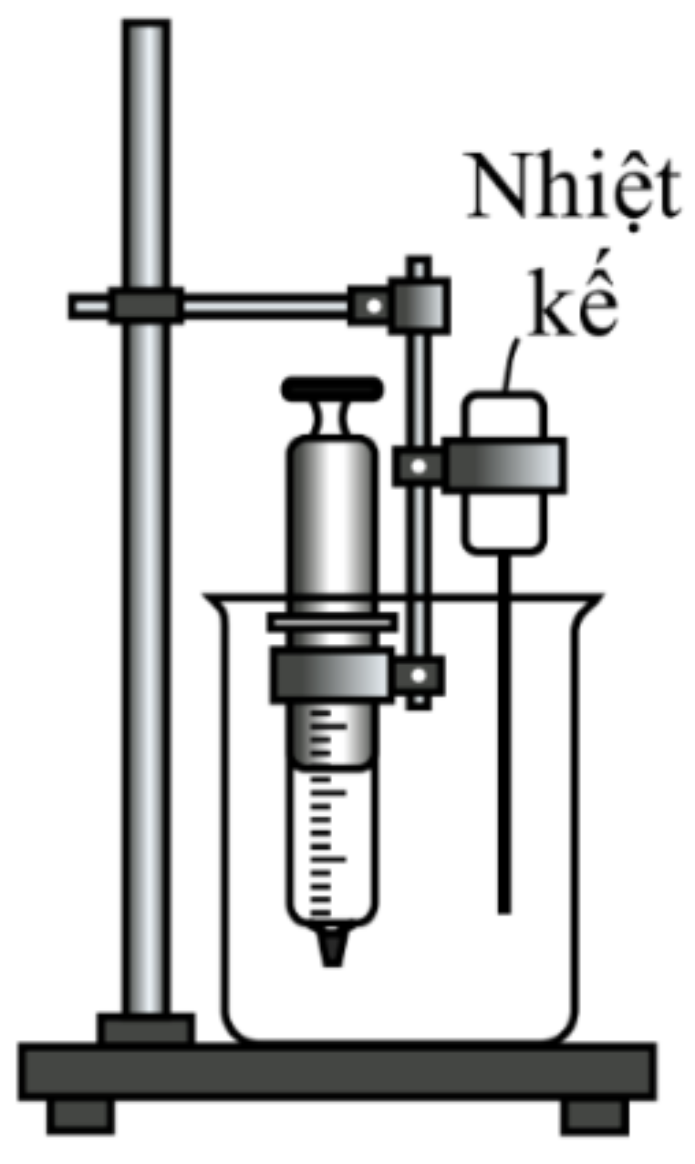
\includegraphics[scale=0.1]{img1/nhiet_ke.png}
	}
\end{ex}

\begin{ex}
	Trong quá trình đẳng áp của một lượng khí, khi nhiệt độ tăng từ $7^{\circ}\text{C}$ lên $147^{\circ}\text{C}$ thì thể tích tăng bao nhiêu lần?
	\choice
	{21}
	{1,5}
	{5,7}
	{7}
\end{ex}

%\begin{ex}
%	Đồ thị nào sau đây \textbf{không} phù hợp với quá trình đẳng áp?
%	\begin{figure}[ht]
%		\centering
%		
\includegraphics[width=0.8\linewidth]{img1/C9.png}
%		\label{fig:placeholder}
%	\end{figure}
%	\choice
%	{Hình 1}
%	{Hình 2}
%	{Hình 3}
%	{Hình 4}
%\end{ex}

%\begin{ex}
%	Đường biểu diễn quá trình đẳng áp của một lượng khí xác định là \textbf{sai}?
%	\begin{figure}[ht]
%		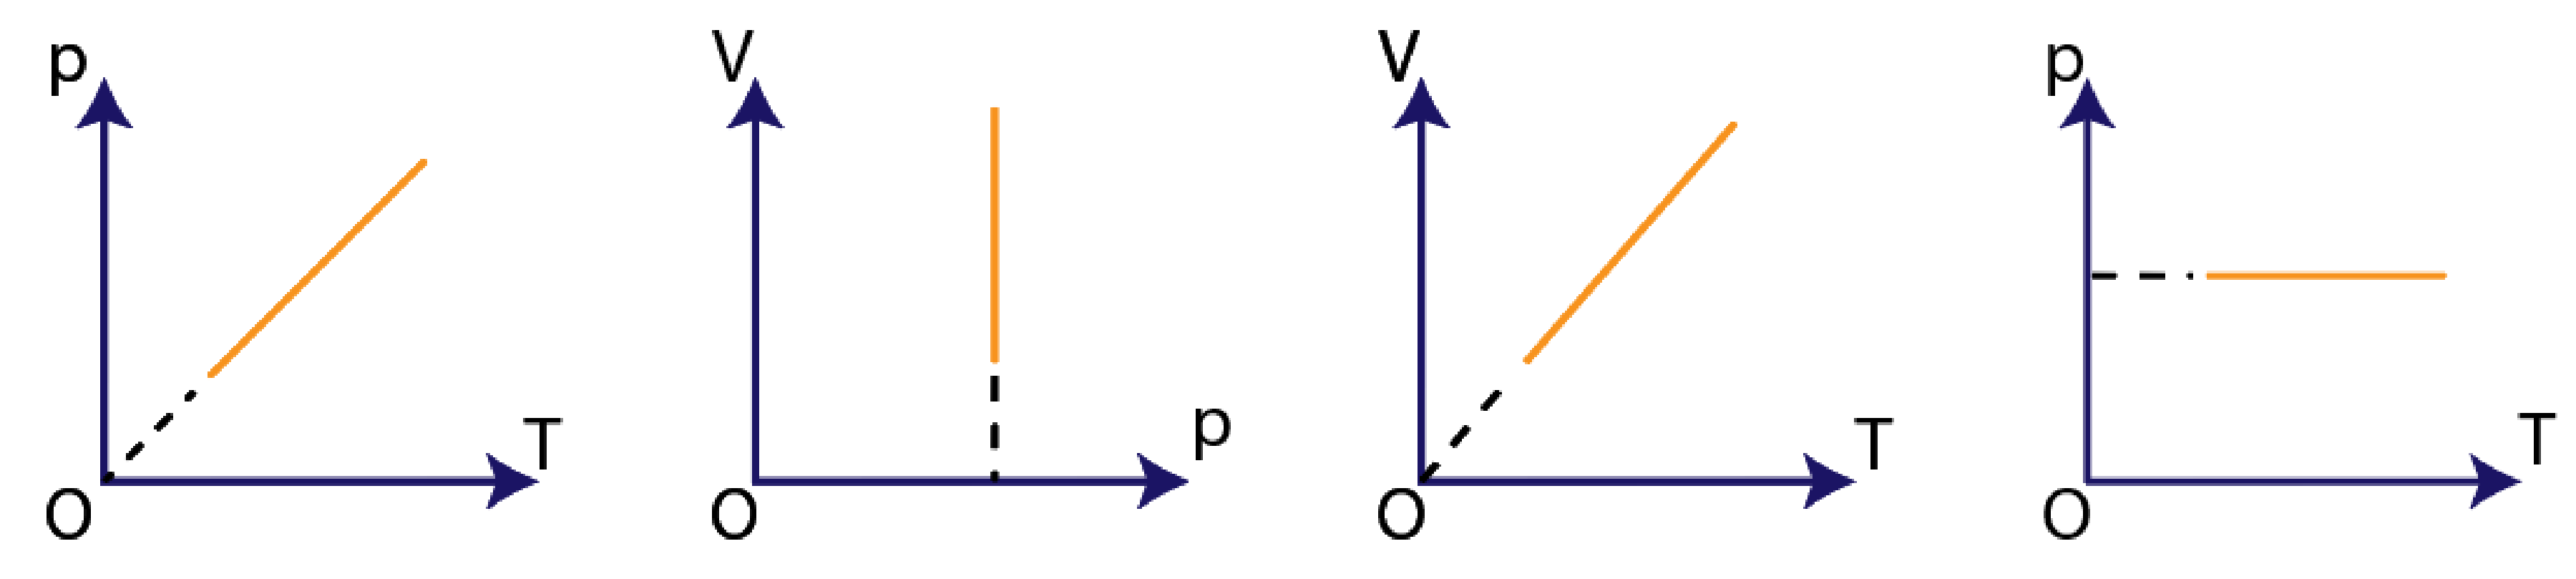
\includegraphics[width=0.9\linewidth]{img1/C10.png}
%		\label{fig:placeholder}
%	\end{figure}
%	\vspace{-0.5cm}
%	\def\dotEX{}
%	\choice
%	{}
%	{}
%	{}
%	{}
%\end{ex}


\begin{ex}
	\immini{Như hình bên, một lượng khí được bịt kín bởi một piston trong xilanh hình trụ đặt thẳng đứng. Piston nhẵn có khối lượng $m$, diện tích mặt cắt ngang là $S$, góc giữa mặt dưới và mặt trên của piston là $\theta$. Biết áp suất khí quyển là $p_{0}$, gia tốc rơi tự do là $g$. Áp suất khí bên trong xilanh là:
	}{
	
\includegraphics[scale=0.3]{img1/xilanh.png}	
	}
	\choice
	{$p_{0} + \dfrac{mgtan\theta}{S}$}
	{$p_{0} + \dfrac{mgsin\theta}{S}$}
	{$p_{0} + \dfrac{mg}{S}$}
	{$p_{0} + \dfrac{mgcos\theta}{S}$}
\end{ex}

\begin{ex}
	\immini{Như hình vẽ, một xilanh đặt thẳng đứng, piston có tiết diện $0,2 \, \text{m}^2$ bịt kín một lượng khí nhất định và một vật rắn trong hình trụ. Khi nhiệt độ là $32^{\circ}\text{C}$, độ cao của piston xo với đáy xilanh là $0,5\, \text{m}$. Khi đun nóng đến $93^{\circ}\text{C}$, xilanh dâng lên $0,05\, \text{m}$. Bỏ qua mọi ma sát và sự thay đổi thể tích vật rắn. Thể tích của vật là:
	}{
		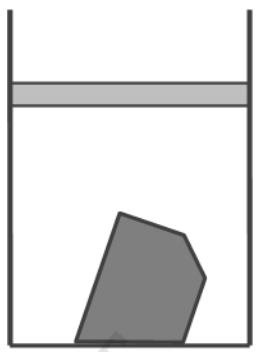
\includegraphics[scale=0.3]{img1/Picture3.png}	
	}
	\choice
	{$0,03 \, \text{m}^3$}
	{$0,02 \, \text{m}^3$}
	{$0,04 \, \text{m}^3$}
	{$0,05 \, \text{m}^3$}
\end{ex}

\begin{ex}
	Khi thổi bong bóng xà phòng, ta quan sát thấy lúc đầu bong bóng bay lên cao rồi dần dần rơi xuống (nếu bong bóng không vỡ giữa chừng).\\	
	(1) Bong bóng xà phòng chịu tác dụng của hai lực chính: trọng lực $P$ hướng thẳng đứng xuống dưới (không đổi) và lực đẩy Acsimet của không khí $F_A$ hướng thẳng đứng lên trên.\\	
	(2) Lúc đầu, khối khí trong bong bóng xà phòng có nhiệt độ cao hơn không khí (hơi thở ra của người có nhiệt độ $37^{\circ}\text{C}$) và $F_A > P$, làm cho bong bóng bay lên.\\	
	(3) Sau đó, bong bóng xà phòng giảm nhiệt độ do tỏa nhiệt lượng ra không khí và thu nhỏ thể tích bong bóng lại nên $F_A$ nhỏ dần đi, còn $P$ không đổi. Đến một lúc nào đó thì $F_A < P$, kết quả là tốc độ đi lên của bong bóng giảm dần rồi từ từ rơi xuống.\\
	Xét tính đúng sai của các mệnh đề trên.
	\choice[2]
	{(1) sai; (2), (3) đúng}
	{(1) đúng; (2), (3) sai}
	{(1), (2) và (3) sai}
	{(1), (2) và (3) đúng}
\end{ex}

\begin{ex}
	Cho đồ thị biến đổi trạng thái của một khối khí lí tưởng xác định, từ trạng thái 1 đến trạng thái 2. Đồ thị nào dưới đây tương ứng với đồ thị trên biểu diễn đúng quá trình biến đổi trạng thái của khối khí này?
	\vspace{-0.75cm}
	\begin{figure}[ht]
		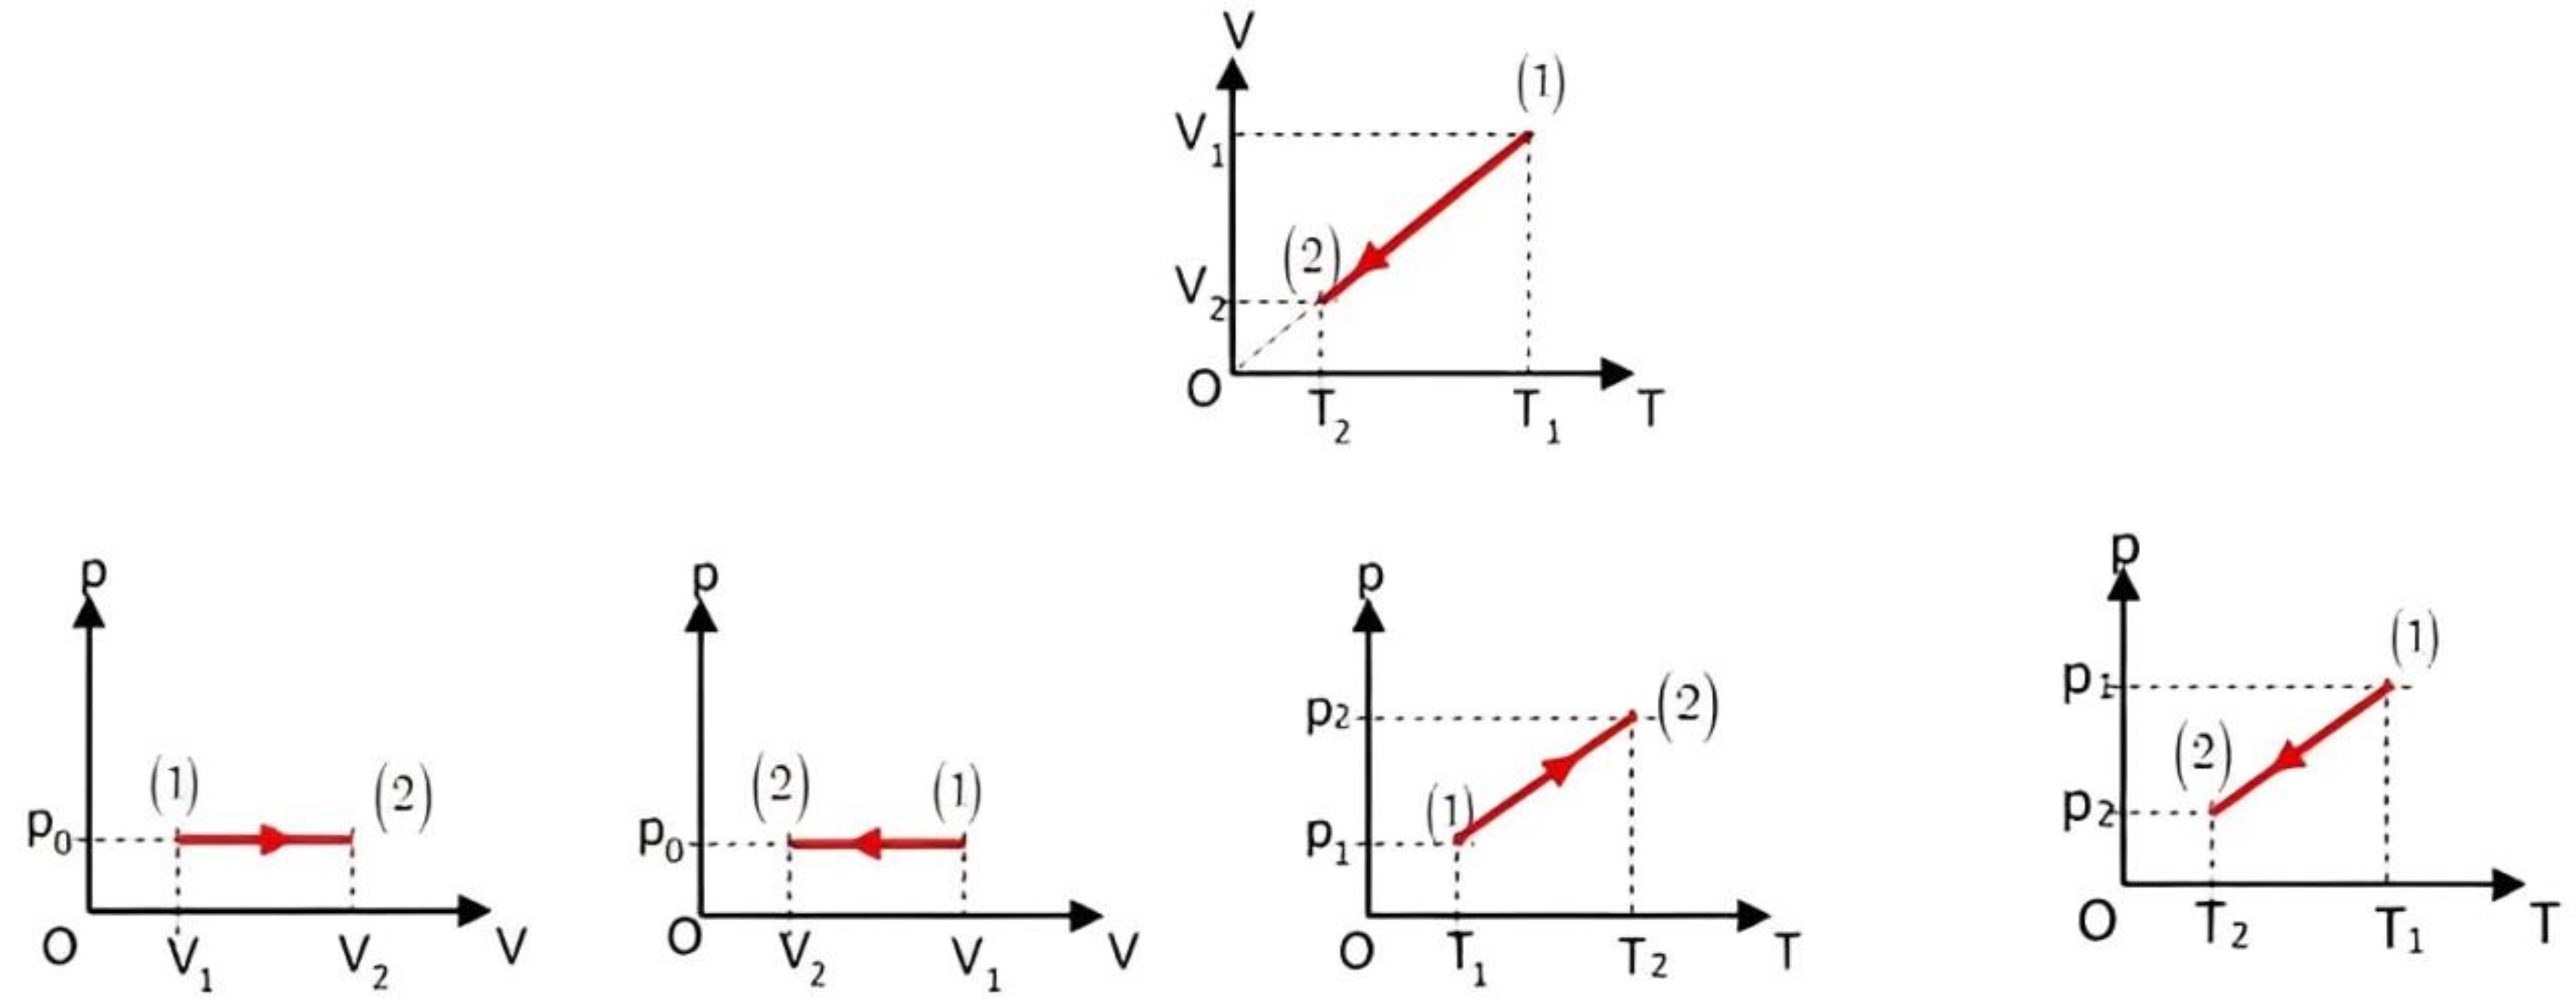
\includegraphics[width=0.95\linewidth]{img1/C11.png}
		\label{fig:placeholder}
	\end{figure}
	\vspace{-0.5cm}
	\def\dotEX{}
	\choice
	{}
	{}
	{}
	{}
\end{ex}

% Câu 5 (Trang 2)
\begin{ex}
	Hiện tượng quả bóng bàn bị bẹp được nhúng vào nước thì phồng lên như cũ liên quan đến đẳng quá trình nào của chất khí?
	\choice
	{Vì trong hiện tượng này, thể tích khí tăng theo nhiệt độ nên liên quan đến quá trình đẳng áp}
	{Vì trong hiện tượng này, áp suất khí tăng theo nhiệt độ nên liên quan đến quá trình đẳng tích}
	{Vì trong hiện tượng này có sự thay đổi thể tích và áp suất nên liên quan đến quá trình đẳng nhiệt}
	{Hiện tượng này không phải là một đẳng quá trình}
\end{ex}

%% Câu 6 (Trang 2)
%\begin{ex}
%	Một mô hình áp kế khí gồm một bình cầu thuỷ tinh có thể tích $270 \text{ cm}^3$ gắn với một ống nhỏ AB nằm ngang có tiết diện $0{,}1 \text{ cm}^2$. Trong ống có một giọt thuỷ ngân. Ở $0^\circ\text{C}$ giọt thuỷ ngân cách A $30 \text{ cm}$. Coi thể tích bình là không đổi. Tính khoảng di chuyển của giọt thuỷ ngân khi hơ nóng bình cầu đến $10^\circ\text{C}$.
%	\choice
%	{$100 \text{ cm}$}
%	{$50 \text{ cm}$}
%	{$150 \text{ cm}$}
%	{$200 \text{ cm}$}
%\end{ex}

% ===========================================================
\noindent\textbf{PHẦN II. Câu trắc nghiệm đúng sai.} Các ý \textbf{a), b), c), d)} ở mỗi câu, chọn đúng hoặc sai.
\setcounter{ex}{0}

% Câu 1 (Trang 2) - Đúng Sai
\begin{ex}
	Một xi lanh đặt nằm ngang chứa $100 \text{ cm}^3$ khí ở nhiệt độ $27^\circ\text{C}$, dưới áp suất bằng áp suất khí quyển bên ngoài $p_0$. Người ta đun nóng khí lên đến $57^\circ\text{C}$ cho pít-tông chuyển động gần như thẳng đều trong xi lanh. Coi ma sát giữa xi lanh và pít-tông không đáng kể.
	\choiceTF
	{\True Quá trình biến đổi trạng thái của khí là đẳng áp với áp suất luôn bằng $p_0$}
	{Thể tích khí trong xi lanh ở $57^\circ\text{C}$ là $120 \text{ cm}^3$}
	{\True Đồ thị biểu diễn quá trình trên theo toạ độ $(V - T)$ là đường thẳng có đường kéo dài đi qua gốc tọa độ}
	{\True Đồ thị biểu diễn quá trình trên theo toạ độ $(p - V)$ là đường thẳng song song với trục $0V$}
\end{ex}

% Câu 2 (Trang 2 + 3) - Đúng Sai
\begin{ex}
	Một nhóm học sinh làm thí nghiệm để xác định mối quan hệ giữa thể tích $V$ và nhiệt độ $T$ của một khối khí lí tưởng xác định khi áp suất khí $p$ không đổi. Thiết bị như hình bên.\\
	\begin{minipage}[t]{0.55\textwidth}
		\resizebox{\linewidth}{!}{%
			\begin{tabular}{|c|>{\centering\arraybackslash}m{4cm}|>{\centering\arraybackslash}m{4cm}|}
				\hline
				Lần đo & Nhiệt độ của khí trong xilanh $t(^{\circ}\text{C})$ & Thể tích khí trong xilanh $V(\text{ml})$ \\
				\hline
				1 & 45 & 75 \\
				\hline
				2 & 41 & 74 \\
				\hline
				3 & 37 & 73 \\
				\hline
				4 & 32 & 72 \\
				\hline
				5 & 28 & 71 \\
				\hline
			\end{tabular}
		}
	\end{minipage}
	\begin{minipage}{0.4\textwidth}
		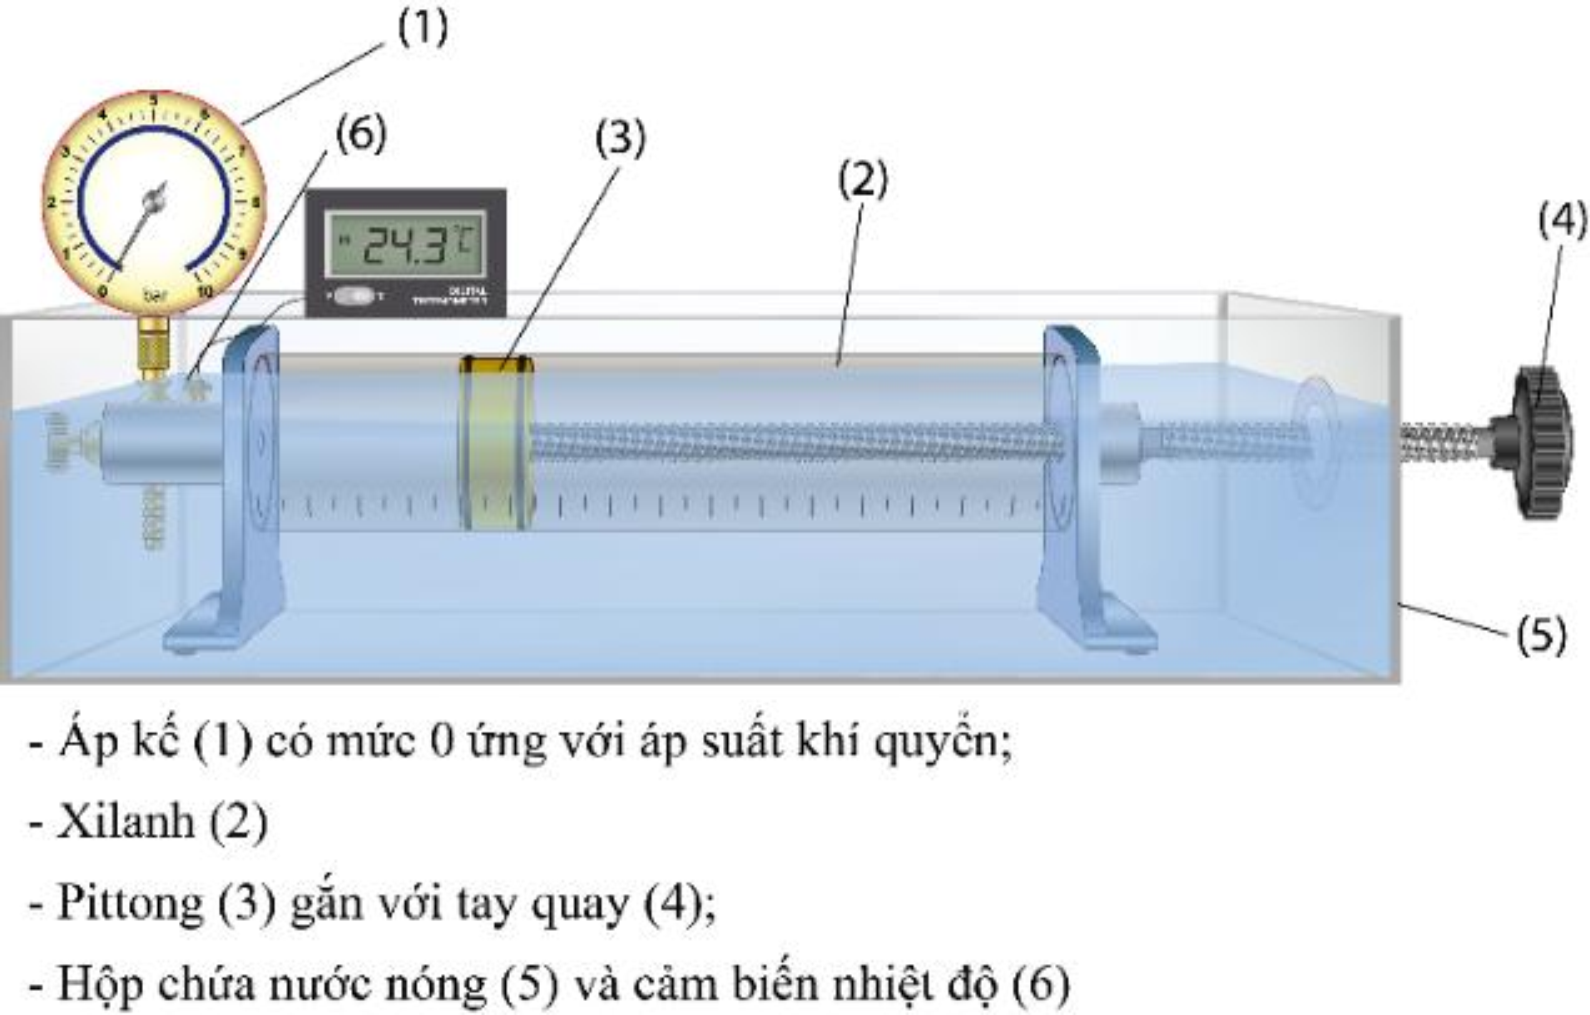
\includegraphics[scale=0.15]{img1/thi_nghiem.png}
	\end{minipage}
	\choiceTF
	{Nhóm học sinh nhận định, $V$ tỉ lệ thuận với $T^2$}
	{\True Nhóm học sinh thực hiện các bước: \\1. Đọc giá trị $V, T$ lúc đầu. \\2. Đổ nước nóng vào hộp chứa cho ngập hoàn toàn xi lanh. Dịch pít-tông từ từ sao cho số chỉ của áp kế không đổi. \\3. Đọc giá trị $V$ và $T$ sau mỗi phút ghi vào bảng bên}
	{Kết quả thí nghiệm đã chứng tỏ nhận định ban đầu là đúng}
	{\True Một số học sinh cho rằng, nếu dịch chuyển nhanh pít-tông thì kết quả thí nghiệm không chính xác}
\end{ex}

% Câu 6 (Trang 2)
\begin{ex}
	Nhóm học sinh làm thí nghiệm, nhúng quả bóng bàn bị xẹp vào nước nóng thì nó phồng lên như khi chưa bị xẹp.
	\choiceTF
	{Một số học sinh nhận định, quá trình biến đổi trạng thái của khí trong quả bóng bàn là quá trình đẳng áp}
	{Một số học sinh giải thích, muốn cho quả bóng phồng lên thì áp lực của không khí bên trong bóng tác dụng lên vỏ bóng phải nhỏ hơn áp lực của không khí bên ngoài và lực đàn hồi của vỏ bóng bị biến dạng}
	{Một số học sinh khác giải thích, áp suất của không khí bên trong bóng phải không đổi để tạo ra áp lực đủ mạnh thắng được áp lực không khí bên ngoài và thắng được lực đàn hồi của vỏ bóng}
	{Một số học sinh khác kết luận, quá trình này số mol khí trong quả bóng không thay thay đổi}
\end{ex}
\newpage
% Câu 7 (Trang 2)
\begin{ex}
	\immini{
	Một khối khí lí tưởng xác định biến đổi từ trạng thái 1 sang trạng thái 2 được biểu diễn trên hệ tọa độ $V - T$ như hình bên.
	\choiceTF
	{Quá trình trên là quá trình làm lạnh đẳng áp}
	{Nhiệt độ của khí ở trạng thái 2 bằng $227^\circ\text{C}$}
	{Quá trình trên, khoảng cách trung bình giữa các phân tử tăng lên}
	{Sau khi hệ đến trạng thái 2 nếu hạ thấp nhiệt độ từ từ thì hệ sẽ đi qua các trạng thái trung gian như quá trình trên đã đi qua}
	}{
	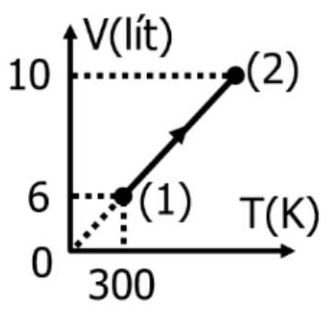
\includegraphics[scale=0.4]{img1/H7.png}
	}
\end{ex}

\begin{ex}
	Một quả bóng bay được bơm khí helium đến thể tích $V_0$ ở nhiệt độ $20^{\circ}\text{C}$. Khi được mang ra ngoài trời nắng, nhiệt độ của khối khí bên trong quả bóng tăng lên đến $40^{\circ}\text{C}$. Áp suất trong quả bóng được coi như không đổi và quả bóng có khả năng dãn nở nhưng chỉ dãn nở tối đa $1{,}101$ lần thể tích ban đầu $V_0$. Coi khối khí bên trong quả bóng là khí lí tưởng.
	\choiceTF
	{Thể tích của quả bóng bay tăng tỉ lệ thuận với nhiệt độ tuyệt đối của khí helium}
	{Nếu quả bóng đi qua vùng không khí nóng có nhiệt độ $50^{\circ}\text{C}$ thì quả bóng sẽ bị vỡ}
	{Nếu cho quả bóng vào vùng nhiệt độ dưới $0^{\circ}\text{C}$ thể tích quả bóng sẽ giảm so với thể tích ban đầu}
	{Khi nhiệt độ khí helium tăng từ $20^{\circ}\text{C}$ đến $40^{\circ}\text{C}$ thể tích của quả bóng bay sẽ tăng gấp đôi}
\end{ex}

\begin{ex}
	\immini{
	Một nhóm học sinh sử dụng bình thuỷ tinh hình cầu gắn với một ống nhỏ AB có tiết diện $0{,}1\,\text{cm}^2$ trong đó có giọt thủy ngân dịch chuyển được để khảo sát quan hệ giữa các thông số trạng thái của khí trong bình. Khi khảo sát ở $20^{\circ}\text{C}$ thì giọt thuỷ ngân cách A $30\,\text{cm}$. Bỏ qua sự nở vì nhiệt của bình. Nhóm học sinh thực hiện các thao tác thí nghiệm và rút ra được các kết luận.
	}{
	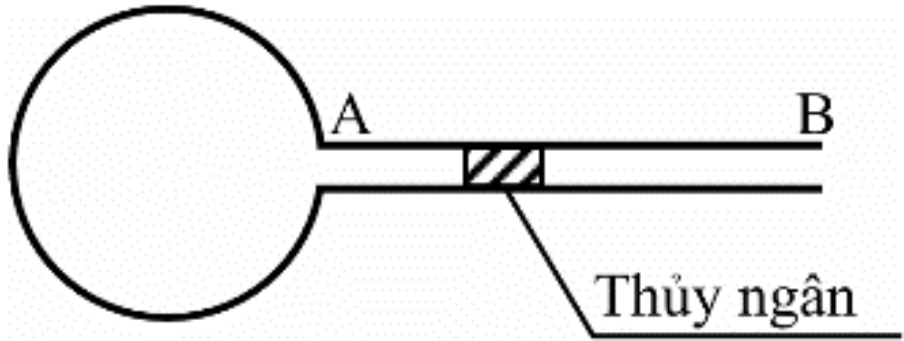
\includegraphics[scale=0.15]{img1/binh_cau.png}
	}
	\choiceTF
	{Hơ nóng khí trong bình thì giọt thuỷ ngân sẽ dịch chuyển lại gần đầu A}
	{Vì không có sự nở vì nhiệt của bình nên quá trình biến đổi trạng thái của khối khí khi bị hơ nóng là quá trình đẳng tích}
	{Hơ nóng khí trong bình thì giọt thủy ngân sẽ dịch chuyển về phía B đến khi áp suất của khí trong bình cân bằng với áp suất khí quyển}
	{Khi nhiệt độ của khí được hơ nóng đến $25^{\circ}\text{C}$ thì giọt thuỷ ngân cách A $50\,\text{cm}$. Phần thể tích của khí chứa trong bình thủy tinh hình cầu là $114{,}2\,\text{cm}^3$}
\end{ex}

\begin{ex}
	Một bình có dung tích $140\,\text{cm}^3$ chứa không khí ở nhiệt độ $147^{\circ}\text{C}$ nối với một ống nằm ngang chứa đầy thuỷ ngân, đầu kia thông với khí quyển. Không khí trong bình được làm lạnh đến $27^{\circ}\text{C}$, coi dung tích bình không đổi và khối lượng riêng của thuỷ ngân là $13{,}6\,\text{g/cm}^3$.
	\choiceTF
	{Ban đầu, cột thuỷ ngân trong ống nằm ngang cân bằng. Áp suất trong bình bằng với áp suất khí quyển}
	{Khi vừa mới giảm nhiệt độ của không khí trong bình, áp suất trong bình giảm và nhỏ hơn áp suất khí quyển làm cho thuỷ ngân bị đẩy vào chiếm một phần thể tích bình chứa}
	{Thể tích của khí sau khi thuỷ ngân chảy vào bình là $100\,\text{cm}^3$}
	{Khối lượng thuỷ ngân chảy vào bình $544$ gam}
\end{ex}

\begin{ex}
	Một ống thuỷ tinh hình trụ thẳng đứng có tiết diện ngang nhỏ, đầu trên hở, đầu dưới kín. Ống chứa một khối khí (coi là khí lí tưởng) có chiều cao $L = 90\,\text{cm}$ được ngăn cách với bên ngoài bởi một cột thuỷ ngân có độ cao $h = 75\,\text{cm}$, mép trên cột thuỷ ngân cách miệng trên của ống một đoạn $l = 10\,\text{cm}$. Nhiệt độ ban đầu của khí trong ống là $t_0 = -3^{\circ}\text{C}$, áp suất khí quyển là $p_0 = 75\,\text{cmHg}$. Người ta thay đổi chậm nhiệt độ của khí trong ống để cột thủy ngân có thể di chuyển trong ống thủy tinh.
	\choiceTF
	{Khi cột thủy ngân chưa trào ra ngoài thì quá trình biến đổi của khí trong ống là quá trình đẳng áp}
	{Đưa nhiệt độ của khí trong ống đến $27^{\circ}\text{C}$ thì mép trên của cột thuỷ ngân vừa chạm miệng trên của ống}
	{Khi được làm nóng, cột thủy ngân sẽ dịch chuyển về phía đầu dưới của ống}
	{Để thuỷ ngân trong ống tràn hết ra ngoài thì phải đưa nhiệt độ của khí trong ống đến nhiệt độ $262{,}5\,\text{K}$}
\end{ex}
\newpage
%======================================================
\noindent\textbf{PHẦN III. Câu trắc nghiệm trả lời ngắn.}
\setcounter{ex}{0}

\begin{ex}
	Khi tăng nhiệt độ của một lượng khí lí tưởng từ $32^\circ\text{C}$ lên $117^\circ\text{C}$ và giữ áp suất khí không đổi thì thể tích khí tăng thêm $1{,}7$ lít. Thể tích lượng khí trước khi tăng nhiệt độ là bao nhiêu lít? Viết đáp số 2 kí tự số.
\end{ex}

% Câu 2 (Trang 3) - Trả lời ngắn
\begin{ex}
	Một mô hình áp kế khí gồm một bình cầu thuỷ tinh có thể tích $270 \text{ cm}^3$ gắn với một ống nhỏ AB nằm ngang có tiết diện $0{,}1 \text{ cm}^2$. Trong ống có một giọt thuỷ ngân. Ở $0^\circ\text{C}$ giọt thuỷ ngân cách A một đoạn a. Khi hơ nóng bình cầu đến $10^\circ\text{C}$ giọt thuỷ ngân di chuyển một đoạn $100 \text{ cm}$. Coi thể tích bình là không đổi. Giá trị a bằng bao nhiêu cm? Viết đáp số 3 kí tự số.
\end{ex}

% Câu 8 (Trang 3)
\begin{ex}
	Một xi lanh có pít-tông kín bên trong có $20 \text{ cm}^3$ khí ở $27^\circ\text{C}$, áp suất $1 \text{ atm}$. Thả pít-tông tự do để khối khí giãn đẳng áp đến thể tích $30 \text{ cm}^3$. Nhiệt độ cuối cùng của khối khí trong xi lanh bằng bao nhiêu $^\circ\text{C}$? Viết đáp số 3 kí tự số.
\end{ex}

% Câu 9 (Trang 3)
\begin{ex}
	Vào những ngày trời nắng nóng, nhiệt độ không khí ngoài sân là $42^\circ\text{C}$, trong khi nhiệt độ không khí trong nhà là $27^\circ\text{C}$. Xem áp suất không khí trong nhà và ngoài sân là như nhau. Gọi $D_1, D_2$ lần lượt là khối lượng riêng của không khí trong nhà và khối lượng riêng của không khí ngoài sân. Biết $D_1 - D_2 = 0{,}086 \text{ kg/m}^3$. Giá trị của $D_1$ bằng bao nhiêu $\text{kg/m}^3$? Lấy chính xác đến 2 chữ số ở phần thập phân.
\end{ex}

\begin{ex}
	Một bình thủy tinh dung tích $14\, \text{cm}^3$ chứa không khí ở nhiệt độ $77^{\circ}\text{C}$ được nối với ống nằm ngang chứa đầy thủy ngân (đầu còn lại để hở). Làm lạnh khí trong bình đến nhiệt độ $27^{\circ}\text{C}$. Tính khối lượng thủy ngân đã chảy vào bình, dung tích bình coi như không đổi. Biết khối lượng riêng của thủy ngân là $13,6\, {\text{g}}/{\text{cm}^3}$
\end{ex}

\begin{ex}
	Khí ở lò thoát ra theo ống khói hình trụ. Ở đầu dưới, khí có nhiệt độ $727^{\circ}\text{C}$ và chuyển động với tốc độ $5\, \text{m/s}$. Hỏi tốc độ của khí ở đầu trên ống (có nhiệt độ $227^{\circ}\text{C}$). Áp suất khí coi như không đổi.
\end{ex}

% =======================================================
\noindent\textbf{PHẦN IV. Tự luận.}
\setcounter{ex}{0}
% Câu 1 (Trang 1) - Dạng điền bảng/vẽ đồ thị (xử lý như câu hỏi tự luận)

% Câu 1 (Trang 3) - Trả lời ngắn
\begin{ex}
	Khi tăng nhiệt độ của một lượng khí lí tưởng từ $32^\circ\text{C}$ lên $117^\circ\text{C}$ và giữ áp suất khí không đổi thì thể tích khí tăng thêm $1{,}7$ lít. Thể tích lượng khí trước khi tăng nhiệt độ là bao nhiêu lít? Viết đáp số 2 kí tự số.
\end{ex}

% Câu 2 (Trang 3) - Trả lời ngắn
\begin{ex}
	Một mô hình áp kế khí gồm một bình cầu thuỷ tinh có thể tích $270 \text{ cm}^3$ gắn với một ống nhỏ AB nằm ngang có tiết diện $0{,}1 \text{ cm}^2$. Trong ống có một giọt thuỷ ngân. Ở $0^\circ\text{C}$ giọt thuỷ ngân cách A một đoạn a. Khi hơ nóng bình cầu đến $10^\circ\text{C}$ giọt thuỷ ngân di chuyển một đoạn $100 \text{ cm}$. Coi thể tích bình là không đổi. Giá trị a bằng bao nhiêu cm? Viết đáp số 3 kí tự số.
\end{ex}
% Câu 3 (Trang 3) - Câu 23
\begin{ex}
	Sử dụng thông tin sau để trả lời các câu 23, câu 24: Một khí cầu có dung tích $336 \text{ m}^3$ và khối lượng vỏ $84 \text{ kg}$ được bơm không khí nóng có nhiệt độ $T_2$ tới áp suất bằng áp suất không khí bên ngoài thì khí cầu vừa bắt đầu bay lên. Lúc này, khối lượng riêng khí trong khí cầu là $D_2$. Biết không khí bên ngoài có nhiệt độ $37^\circ\text{C}$, áp suất $1 \text{ atm}$ và khối lượng riêng là $1{,}29 \text{ kg/m}^3$.
	\begin{listEX}
		\item Giá trị $D_2$ bằng bao nhiêu $\text{kg/m}^3$? 
		\item Giá trị $T_2$ bằng bao nhiêu kelvin?	
	\end{listEX}
\end{ex}

\end{document}